\question
Вы разрабатываете модель процессора с помощью коммутационных схем. Вам необходимо реализовать проверки условных конструкций: обработчику поступает на вход 4 битное число (от 0 до 15 в десятичной системе), в зависимости от заданных условий он возвращает 1 или 0.

Схематически это можно представить так: есть 4 входа (1 вход на каждый бит, биты поступают на входы слева направо), 1 выход:
\\
\begin{figure}[h]

\begin{minipage}[h]{0.55\linewidth}
\end{minipage}
\begin{minipage}[h]{0.45\linewidth}
\center{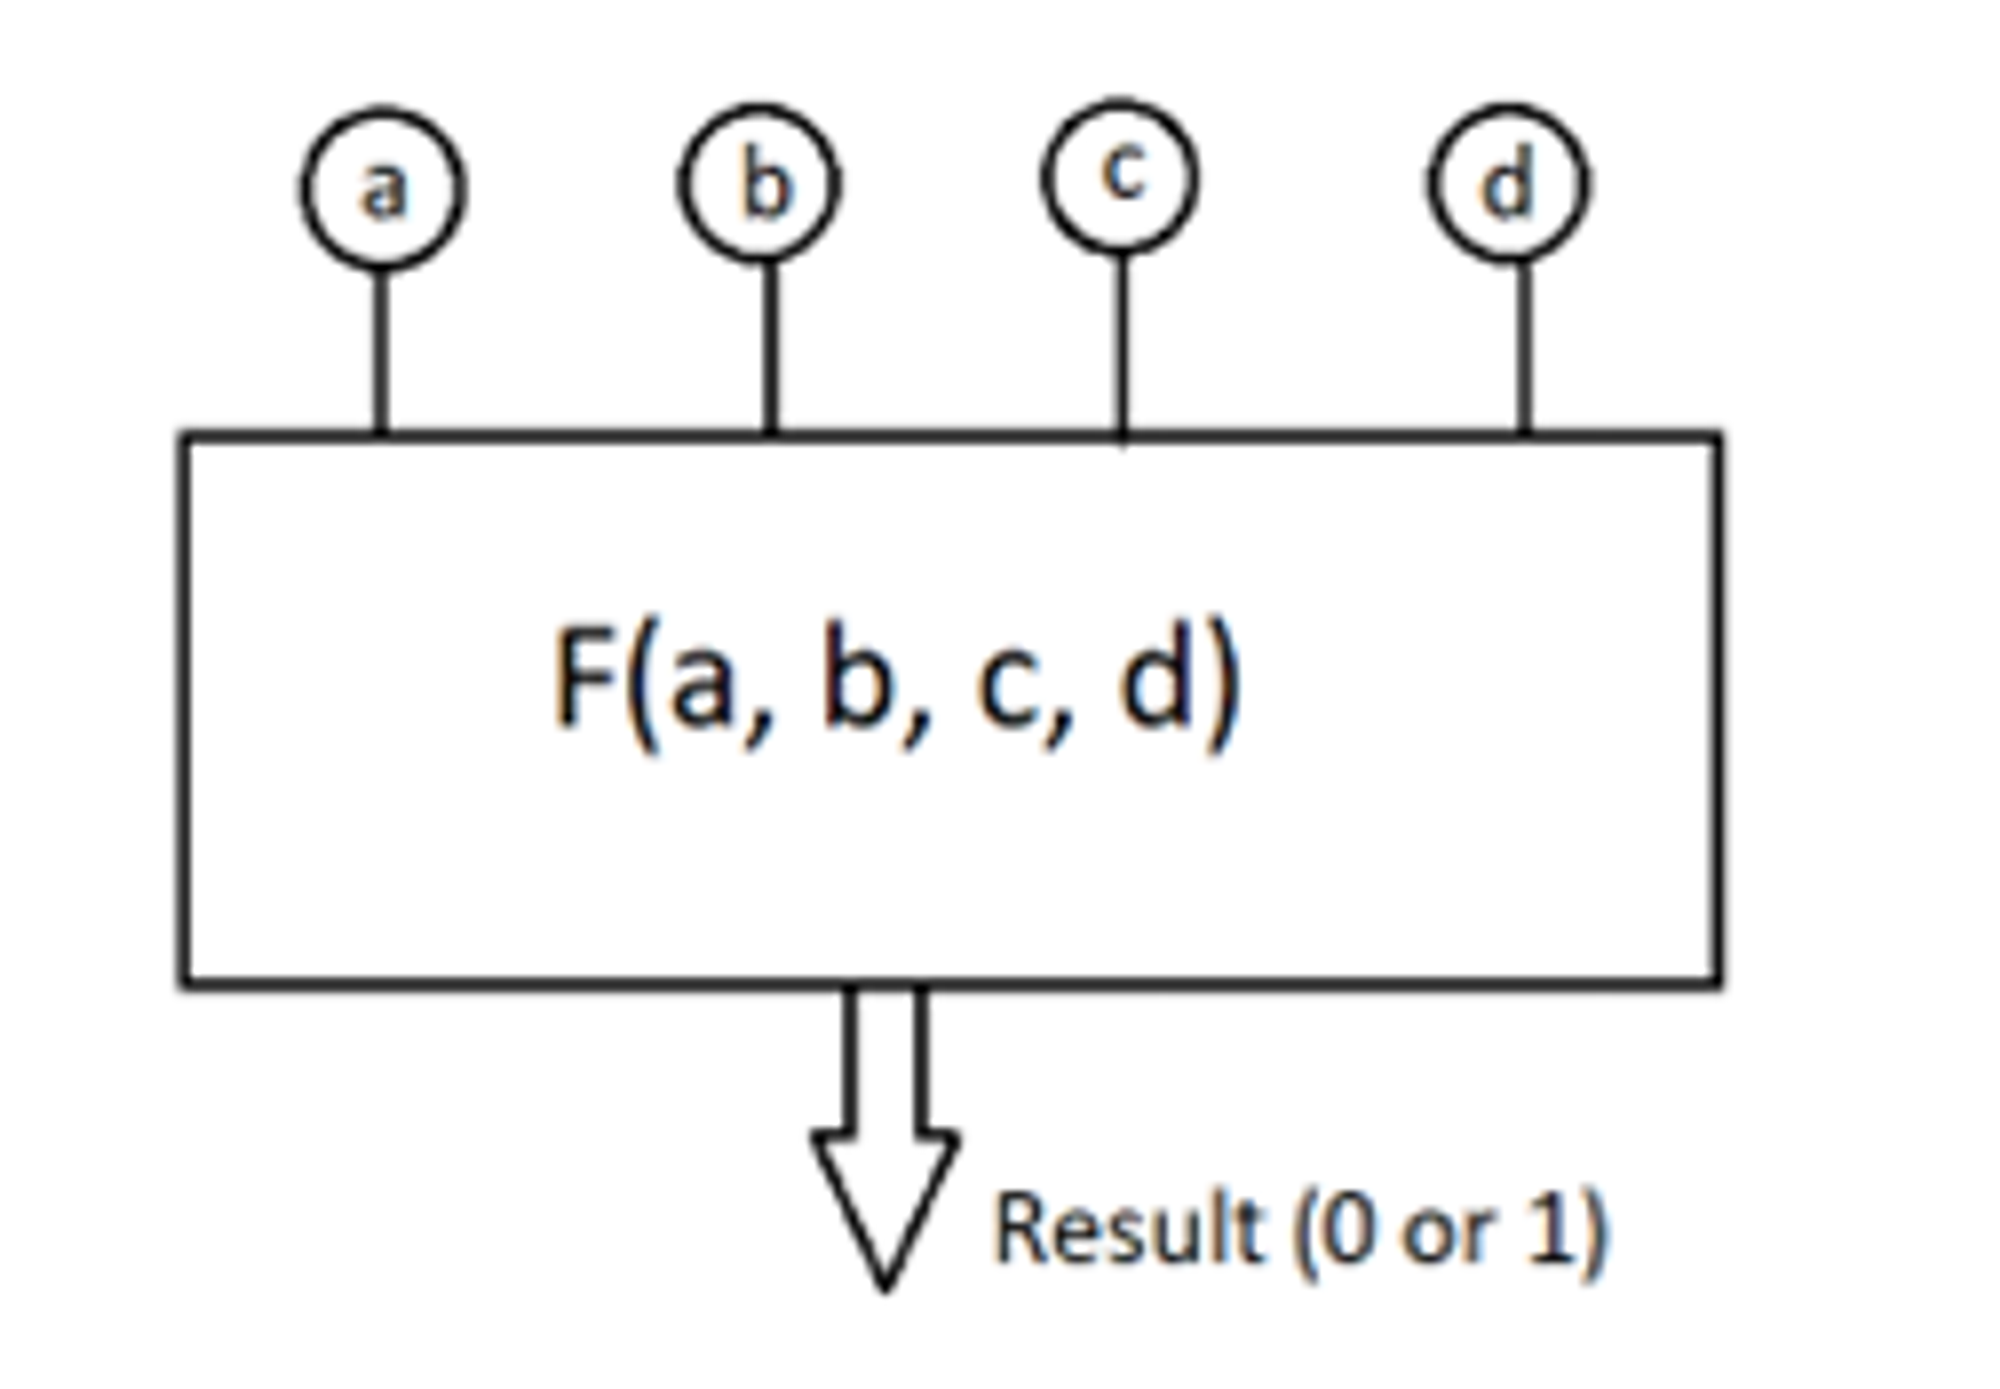
\includegraphics[width=0.7\textwidth]{pic/811.png} }
\end{minipage}
\end{figure}

Реализуйте обработку следующих условий, спроектировав коммутационные схемы:
\begin{enumerate}
    \item Вывести 1, если число на входе делится на 4 (иначе 0)
    \item Вывести 1, если число на входе больше 6, но меньше 12 (иначе 0)
    \item Вывести 1, если число на входе больше 4, и при этом нечётное (иначе 0)
\end{enumerate}

---------------

Автор -- Тимур Гонтарь, М3206